\twocolumn
\begin{figure}[h]
    \centering
    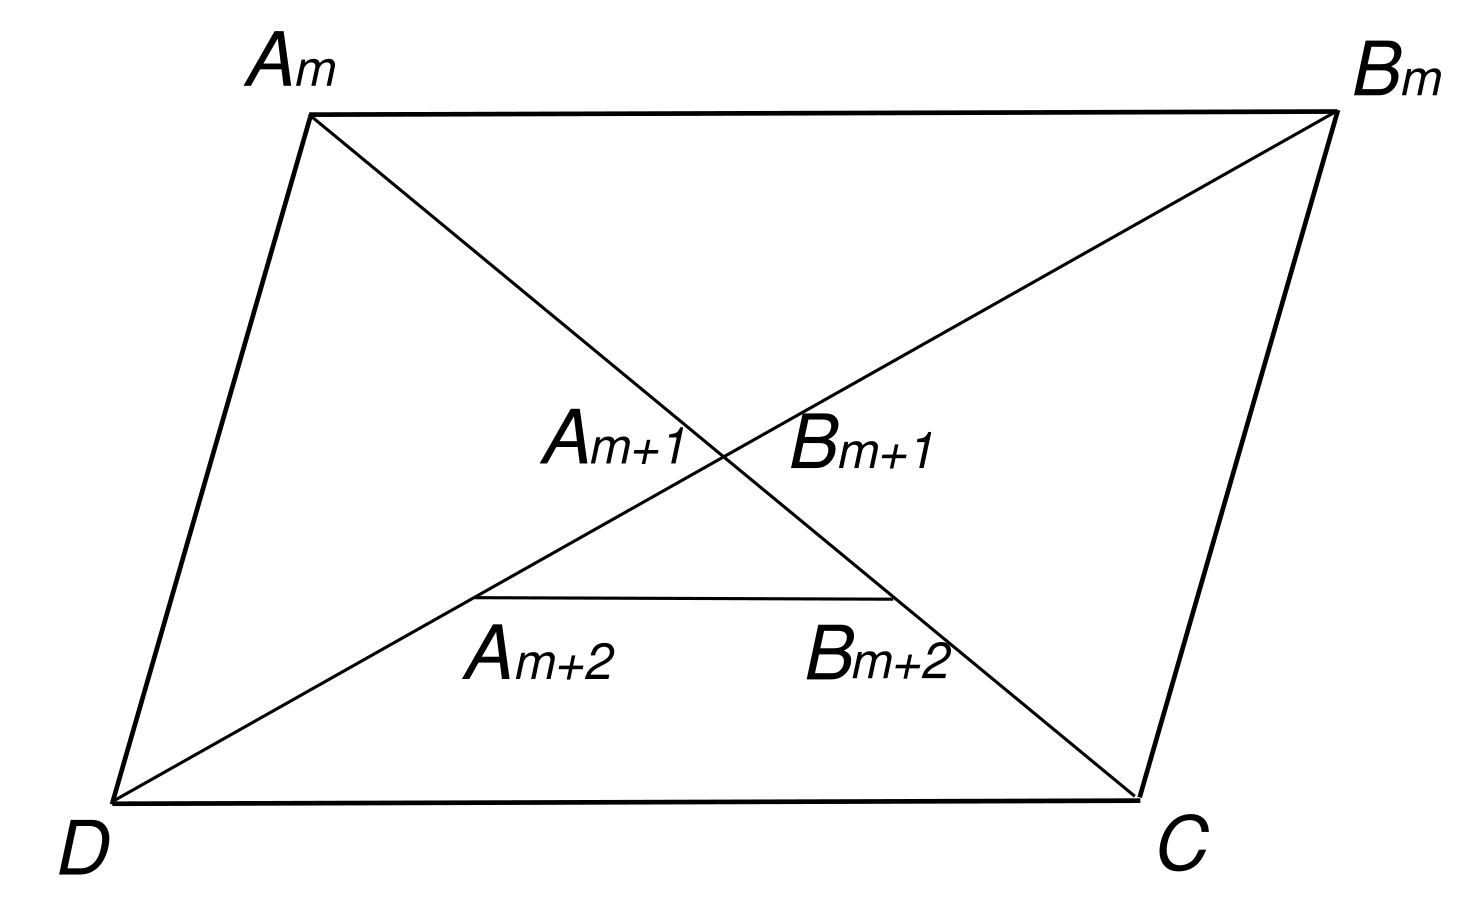
\includegraphics[width=\linewidth]{piped.png}
    \begin{flushleft}
    \textbf{Рис. 5.}
    \end{flushleft}
\end{figure}
К сожалению, некоторые читатели пишут: <<Поскольку последовательность не монотонная, она не стремится к пределу>>. Это рассуждение, конечно, неверно. Докажем строго, пользуясь определением предела